\chapter{粒子扩散}\label{ch:b2:particle-diffusion}

将一小块染料晶体投入静水中并加以观察：一团有色的云雾
在其周围形成、扩大、边缘逐渐柔化，并不断扩展——
一分钟内扩散约一毫米，一小时内扩散约一厘米，一周内
遍布整个玻璃容器。没有任何外力推动染料，它是被分子不停的
无规碰撞携带的，每个粒子因此做无规行走，
平均而言，由粒子密集处迁向稀疏处。
这就是\emph{扩散}，是最慢也最普遍的一种输运方式：
它为每个细胞输送氧气，为每个晶体管掺入硼，
使钢通过渗碳而变硬，也让香水在房间中弥散——不过，
正如我们将看到的，所需时间未必如人们想象的那样短。本章给出
扩散的定律（菲克定律）、由粒子数守恒导出的方程、
其特征解与时间尺度（$L \sim \sqrt{Dt}$），以及它的
微观起源：无规行走——这也解释了为何扩散方程
与力学中的每个方程都不同，它能区分时间的方向。
下一章将把这些内容全部用于热传导。

\begin{omfigure}
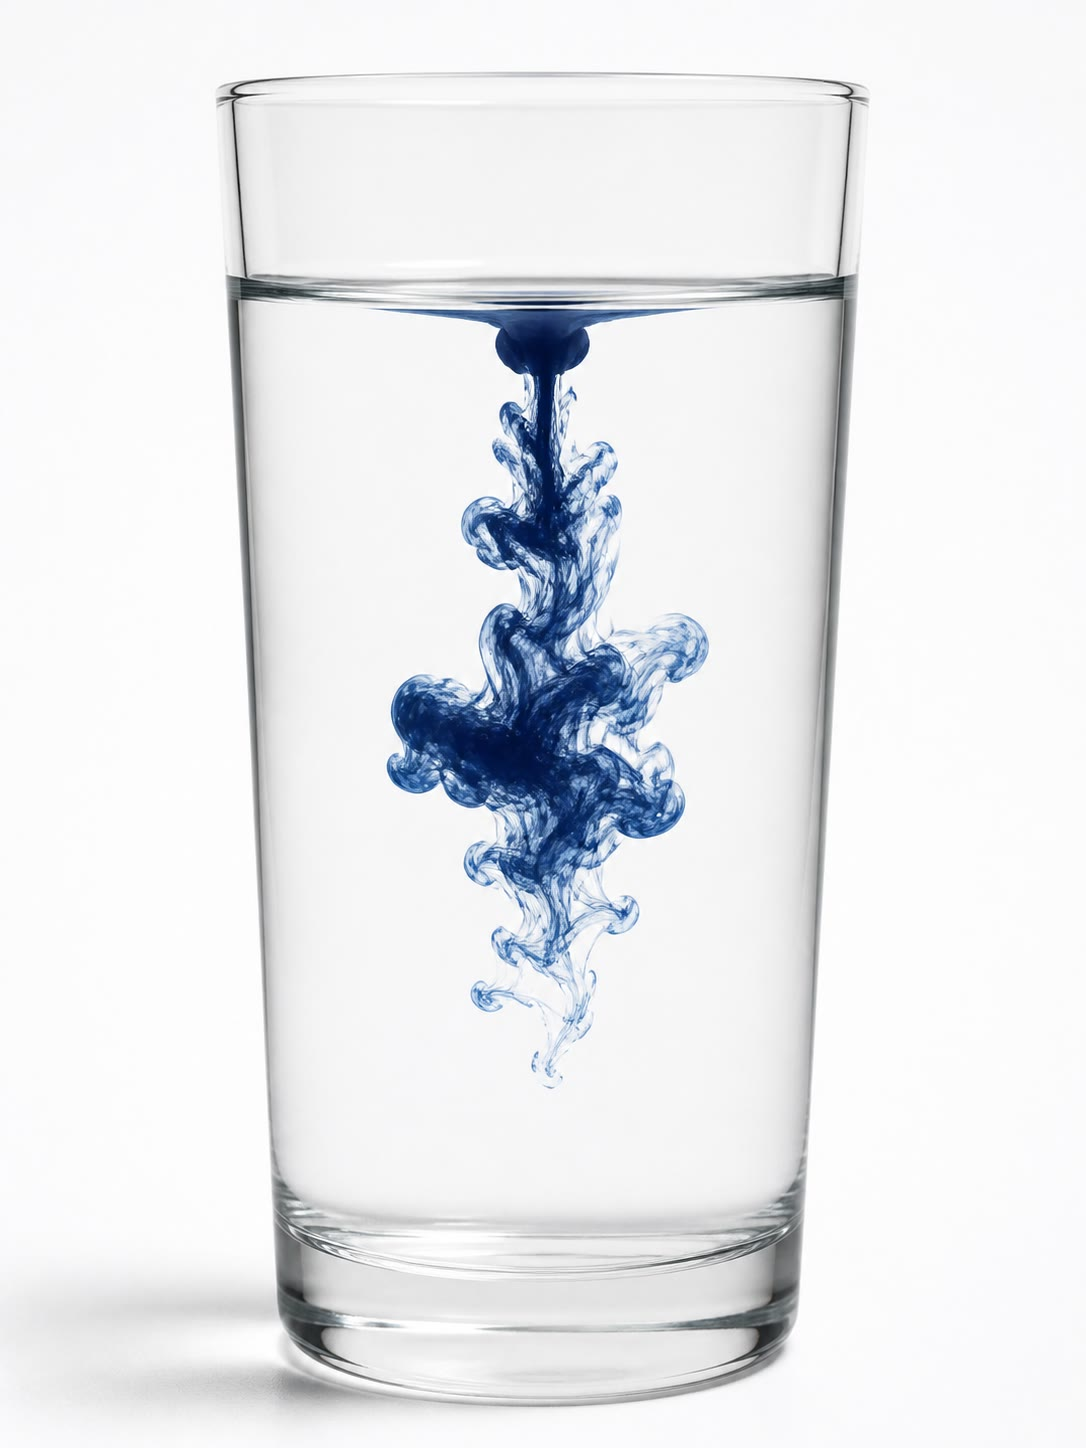
\includegraphics[width=0.58\linewidth]{images/book4/ai/b4-24-ink-drop-water.jpg}

{\small 墨水滴入静水中：清晰的墨云模糊并扩散，
分子扩散使其在一分钟内扩散数毫米，
一小时内可达数厘米。}
\end{omfigure}

\section{数密度、通量与菲克定律}

\begin{definition}[数密度与粒子流密度]\label{def:b2:particle-diffusion:flux}
对某一种粒子（分子、离子、固体中的原子）而言，
\emph{数密度}\index{数密度} $n(M,t)$ 是
$M$ 附近单位体积内的粒子数（单位 \unit{m^{-3}}；摩尔浓度
为 $c = n/N_A$）。\emph{粒子流
密度}\index{粒子流密度} $\vect{j}_N$ 为一矢量，
满足：穿过定向面元的粒子数
$\dd\vect S$ 在 $\dd t$ 内为 $\vect{j}_N\cdot\dd\vect S\,\dd t$（单位
\unit{m^{-2}.s^{-1}}）：经曲面 $S$ 的\emph{粒子通量}为
$\Phi_N = \iint_S \vect{j}_N\cdot\dd\vect S$，即每秒
穿过 $S$ 的粒子数。若粒子由以 $\vect v$ 运动的流体携带，
则 $\vect{j}_N = n\vect v$（对流）；扩散则是静止流体中
仍然存在的输运方式。
\end{definition}

\begin{theorem}[菲克定律]\label{thm:b2:particle-diffusion:fick}
在静止的介质中，若数密度不均匀，
则出现粒子流，其与数密度的
梯度成正比、方向相反：
\[
\vect{j}_N = -D\,\vect{\operatorname{grad}}\,n ,
\]
式中\emph{扩散系数}\index{扩散系数}
$D > 0$（单位 \unit{m^2/s}）取决于扩散粒子种类、介质
及温度。粒子沿数密度梯度\emph{下降}，即由稠密处
流向稀疏处，迁移速率由 $D$ 决定。
\end{theorem}

\begin{proof}
唯象定律（经验规律，类似欧姆定律）：梯度较小时
与梯度呈线性关系，在各向同性介质中具有各向同性，
并具有实验所给定的符号。无规行走模型
在\cref{sec:b2:particle-diffusion:microscopic}中导出了它，并连同 $D$ 一起，
由分子运动得出。
\end{proof}

\begin{example}[$D$ 的数量级]\label{ex:b2:particle-diffusion:orders}
气体：$D \sim \qty{1e-5}{m^2/s}$（空气中的水蒸气
\qty{2.5e-5}{m^2/s}，香水分子为 \qty{5e-6}{m^2/s}）。液体：
$D \sim \qty{1e-9}{m^2/s}$（水中的氧气 \qty{2e-9}{m^2/s}，糖
\qty{5e-10}{m^2/s}，蛋白质 \qty{1e-10}{m^2/s}）。固体：很小，并且
随温度急剧增大，$D = D_0\,\eu^{-E_{\text{a}}/k_BT}$
（硼在硅中：在 \qty{1100}{\celsius} 时为 \qty{1.5e-17}{m^2/s}，
在室温下小到无法测量——这正是晶体管制成后
其掺杂分布可保持数十年的原因）。从气体到液体，相差四个
数量级；从液体到固体则相差八个或更多数量级。
\end{example}

\section{粒子守恒与扩散方程}

\begin{theorem}[局域粒子数守恒]\label{thm:b2:particle-diffusion:balance}
若粒子既不产生也不湮灭，
\[
\frac{\partial n}{\partial t} + \operatorname{div}\vect{j}_N = 0 ;
\]
若存在源，单位体积、单位时间内产生 $\sigma$ 个粒子
（如化学反应、吸收），则 $\partial_t n +
\operatorname{div}\vect{j}_N = \sigma$。一维情形（数密度与
粒子流仅依赖于 $x$）：$\partial_t n + \partial_x j_N = 0$。
\end{theorem}

\begin{proof}
取位于 $x$ 与 $x + \dd x$ 之间、截面积为 $S$ 的薄片：其中含
$n\,S\,\dd x$ 个粒子。在 $\dd t$ 内，经左侧面进入的粒子数为 $j_N(x)S\,\dd t$，
经右侧面离开的粒子数为 $j_N(x + \dd x)S\,\dd t$，于是
$\partial_t n\,S\,\dd x\,\dd t = -(j_N(x+\dd x) - j_N(x))S\,\dd t =
-\partial_x j_N\,\dd x\,S\,\dd t$。在三维情形下，对小盒作同样计数
即得散度（每单位体积的闭合曲面
流出通量，见\cref{ch:b2:maxwell-equations}），或直接：对任一固定
体积 $V$，$\dd/\dd t \iiint_V n\,\dd\tau = -\iint_{\partial V}
\vect{j}_N\cdot\dd\vect S = -\iiint_V \operatorname{div}\vect{j}_N\,\dd\tau$
由奥斯特罗格拉茨基定理得到。
\end{proof}

\begin{omfigure}
\begin{tikzpicture}[scale=1.0, >=stealth]
  \draw[thick] (0,0) rectangle (5,2);
  \fill[omDef!12] (2.2,0) rectangle (2.9,2);
  \draw[omDef, thick] (2.2,0) -- (2.2,2);
  \draw[omDef, thick] (2.9,0) -- (2.9,2);
  \node[font=\scriptsize, below left] at (2.25,0) {$x$};
  \node[font=\scriptsize, below right] at (2.85,0) {$x + \dd x$};
  \draw[->, omExo, very thick] (1.0,1) -- (2.1,1) node[midway, above, font=\scriptsize] {$j_N(x)$};
  \draw[->, omExo, very thick] (3.0,1) -- (4.1,1) node[midway, above, font=\scriptsize] {$j_N(x + \dd x)$};
  \node[font=\scriptsize] at (2.55,1.6) {$n$};
  \node[font=\scriptsize, right] at (5.1,1) {截面 $S$};
  \draw[->] (0,-0.7) -- (5.5,-0.7) node[right, font=\scriptsize] {$x$};
\end{tikzpicture}

{\small 一维平衡：$x$ 与 $x + \dd
x$ 之间的薄层，从左侧流入的量使其增加，从右侧流出的量使其减少；
二者之差即为内部 $n$ 的变化量。}
\end{omfigure}

\begin{theorem}[扩散方程]\label{thm:b2:particle-diffusion:equation}
结合菲克定律与上述平衡关系，对均匀的 $D$，
\[
\frac{\partial n}{\partial t} = D\,\Delta n + \sigma ,
\qquad\text{在一维情形下}\quad
\frac{\partial n}{\partial t} = D\,\frac{\partial^2 n}{\partial x^2} + \sigma .
\]
该\emph{扩散方程}\index{扩散方程}是线性的
（解可以叠加），对时间为一阶，对空间为二阶，
——它不是波动方程：没有传播速度，而具有
一种长度与时间之间的特征关系，
\[
L \sim \sqrt{D t}, \qquad t \sim \frac{L^2}{D} :
\]
扩散距离加倍，所需时间变为四倍。
\end{theorem}

\begin{proof}
$\partial_t n = -\operatorname{div}(-D\,\vect{\operatorname{grad}}\,n) +
\sigma = D\operatorname{div}\vect{\operatorname{grad}}\,n + \sigma = D\Delta
n + \sigma$。就尺度而言，比较 $n/t$ 与 $Dn/L^2$。
\end{proof}

\begin{remark}[扩散是不可逆的]\label{rem:b2:particle-diffusion:irreversible}
将 $t$ 换为 $-t$，在波动方程 $\partial_t^2 u = c^2
\partial_x^2 u$ 中，方程保持不变：波的影片倒放，仍是
一个可能的波。对扩散方程做同样变换，则左侧的符号
翻转：$n(x,-t)$ 并\emph{不}是解。一团
扩散是自然的；一团自发聚成晶体
则不然——扩散有一个时间箭头，即热力学第二定律的
方向（\cref{ch:b2:heat-conduction} 计算了它产生的熵）。
方程还表明，扩散使分布趋于平滑：在 $n$ 局部
取极大值处（$\partial_x^2 n < 0$）它减小，取极小值处它
增大。
\end{remark}

\begin{example}[需要多长时间？]\label{ex:b2:particle-diffusion:times}
$t \sim L^2/D$。氧气穿过一个细胞，在水中 $L = \qty{10}{\micro m}$：
$10^{-10}/2 \times 10^{-9} = \qty{0.05}{s}$ ——扩散足以轻松地为细胞
供氧；穿过 \qty{1}{mm} 的组织：\qty{500}{s} ——太慢了，这就是
这就是为什么没有血管的活体组织
厚度都不能超过毫米的几分之一。一杯未搅拌的茶中的糖，$L = \qty{5}{cm}$：
$2.5 \times 10^{-3}/5 \times 10^{-10} = 5 \times 10^6\,\unit{s}$，两个月
——需要搅拌。仅靠扩散使香水穿过房间，距离 \qty{5}{m}
空气中：$25/10^{-5} = \qty{3e6}{s}$，约一个月；但你在一分钟内就能闻到，
因为空气在流动：\emph{对流}负责输运，扩散只
完成最后几毫米的距离。
\end{example}

\section{特征解}

\begin{proposition}[定态情形：薄膜]\label{prop:b2:particle-diffusion:membrane}
两个粒子库分别保持 $n_1$ 与 $n_2$，二者之间隔着一层
厚度为 $e$、面积为 $S$ 的薄膜，定态密度是线性的，
\[
n(x) = n_1 + (n_2 - n_1)\frac{x}{e}, \qquad
j_N = D\,\frac{n_1 - n_2}{e}, \qquad
\Phi_N = \frac{n_1 - n_2}{R_{\text{d}}}, \quad R_{\text{d}} = \frac{e}{DS}:
\]
薄膜具有\emph{扩散电阻} $e/DS$，正如导线具有
$\ell/\gamma S$ ——串联电阻相加，一层很薄的薄膜，
若 $D$ 很小，仍可能起主导作用。
\end{proposition}

\begin{proof}
定态、一维、无源：$\partial_x^2 n = 0$，故 $n$ 为
线性函数；$j_N = -D\,\dd n/\dd x$ 为均匀的。
\end{proof}

\begin{proposition}[定态情形：球形几何]\label{prop:b2:particle-diffusion:sphere}
在半径为 $a$ 的球体周围，其表面保持 $n_0$，
在远处 $n \to 0$ 的介质中，定态密度为
\[
n(r) = n_0\,\frac{a}{r}, \qquad
\Phi_N = 4\pi D a\,n_0 :
\]
释放（或吸收，符号相反）的总粒子流随
球的\emph{半径}增大，而不随表面增大——
扩散汇的几何形状与一个静电电容的相同。
\end{proposition}

\begin{proof}
$\Delta n = \frac{1}{r^2}\frac{\dd}{\dd r}(r^2\,\dd n/\dd r) = 0$ 给出
$n = A + B/r$；边界条件确定 $A = 0$，$B = n_0 a$；于是
$\Phi_N = -4\pi r^2 D\,\dd n/\dd r = 4\pi D n_0 a$，对任意 $r$ 均成立（
定态情形下无积累）。
\end{proof}

\begin{omfigure}
\begin{tikzpicture}
  \begin{axis}[omaxis, width=5.6cm, height=4.2cm, xmin=-0.3, xmax=1.4, ymin=0, ymax=1.3,
    xlabel={$x/e$}, ylabel={$n/n_1$}, xtick={0,1}, ytick={1}, clip=false]
    \addplot[omDef, thick, domain=0:1] {1-0.7*x};
    \draw[dashed] (axis cs:1,0) -- (axis cs:1,0.3);
    \node[font=\scriptsize, anchor=west] at (axis cs:1.03,0.3) {$n_2$};
    \node[font=\scriptsize, omExo, anchor=west] at (axis cs:0.3,1.0) {$j_N = D(n_1 - n_2)/e$};
    \draw[->, omExo, thick] (axis cs:0.3,0.45) -- (axis cs:0.7,0.45);
  \end{axis}
  \begin{axis}[omaxis, width=5.6cm, height=4.2cm, xmin=0, xmax=5, ymin=0, ymax=1.3, xshift=5.9cm,
    xlabel={$r/a$}, ylabel={$n/n_0$}, xtick={1,2,3,4}, ytick={1}, clip=false]
    \addplot[omDef, thick, domain=1:5, samples=60] {1/x};
    \draw[dashed] (axis cs:1,0) -- (axis cs:1,1);
    \node[font=\scriptsize, omExo] at (axis cs:3,0.6) {$n = n_0 a/r$};
  \end{axis}
\end{tikzpicture}

{\small 稳态分布。左：穿过薄膜时，密度
呈线性变化，粒子流均匀。右：绕球体时，密度
按 $1/r$ 下降；总粒子流 $4\pi D a n_0$ 与
半径成正比。}
\end{omfigure}

\begin{proposition}[扩散的高斯解]\label{prop:b2:particle-diffusion:gaussian}
单位面积上 $N$ 个粒子于 $t = 0$ 时释放在无限介质的
平面 $x = 0$ 上，其扩散为
\[
n(x,t) = \frac{N}{\sqrt{4\pi D t}}\,\exp\Big(-\frac{x^2}{4Dt}\Big) :
\]
高斯分布，标准差为 $\sigma(t) = \sqrt{2Dt}$，
面积恒为 $N$（粒子数守恒），峰值 $\propto
1/\sqrt t$ 随之减小。三维情形下，在一点释放 $N$ 个粒子，
其扩散为 $n = N\,(4\pi Dt)^{-3/2}\exp(-r^2/4Dt)$，且 $\langle r^2
\rangle = 6Dt$。若粒子脉冲释放于半空间的\emph{表面}，
（粒子不能离开半空间），则分布为上式的两倍，
对 $x > 0$ 成立。
\end{proposition}

\begin{proof}
代入：取 $u = x^2/4Dt$，则 $\partial_t n = n\,(-1/2t + u/t)$，且
$D\,\partial_x^2 n = D\,n\,(-1/2Dt + x^2/4D^2t^2) = n\,(-1/2t + u/t)$；
两者相等。归一性 $\int n\,\dd x = N$ 由 $\int
\eu^{-x^2/4Dt}\dd x = \sqrt{4\pi Dt}$ 得出，又 $\int x^2 n\,\dd x/N = 2Dt$。
给定初始脉冲时，解的唯一性在本阶段不加证明地承认。
\end{proof}

\begin{omfigure}
\begin{tikzpicture}
  \begin{axis}[omaxis, width=9cm, height=4.8cm, xmin=-4.2, xmax=4.2, ymin=0, ymax=1.05,
    xlabel={$x/\sqrt{2Dt_1}$}, ylabel={$n$}, ytick=\empty, xtick={-4,-2,2,4}, clip=false,
    legend style={font=\scriptsize, at={(0.97,0.95)}, anchor=north east, draw=none, fill=none}]
    \addplot[omDef, thick, domain=-4.2:4.2, samples=100] {exp(-x*x/2)};
    \addlegendentry{$t_1$}
    \addplot[omThm, thick, domain=-4.2:4.2, samples=100] {0.5*exp(-x*x/8)};
    \addlegendentry{$4t_1$}
    \addplot[omExo, thick, domain=-4.2:4.2, samples=100] {0.25*exp(-x*x/32)};
    \addlegendentry{$16t_1$}
  \end{axis}
\end{tikzpicture}

{\small 三个时刻的高斯解：宽度随
$\sqrt t$ 增大，峰值随 $1/\sqrt t$ 下降，面积（粒子数）
保持不变。}
\end{omfigure}

\begin{proposition}[表面浓度恒定]\label{prop:b2:particle-diffusion:erfc}
起初为空的半空间 $x > 0$，其表面保持
密度 $n_0$，自 $t = 0$ 起（例如与能溶解该气体的固体接触的气体），
逐渐被填充，其分布为
\[
n(x,t) = n_0\,\operatorname{erfc}\Big(\frac{x}{2\sqrt{Dt}}\Big),
\qquad
\operatorname{erfc}(u) = \frac{2}{\sqrt\pi}\int_u^{\infty}\eu^{-s^2}\dd s,
\]
\emph{余误差函数}，从 $1$（$u =
0$ 时）降至 $0.16$（$u = 1$ 时）、$0.005$（$u = 2$ 时）：穿透深度仍为
$\sim 2\sqrt{Dt}$，且单位面积吸收的粒子总数
为 $2n_0\sqrt{Dt/\pi}$。
\end{proposition}

\begin{proof}
设 $n = f(u)$，其中 $u = x/2\sqrt{Dt}$，则方程化为
$f'' + 2uf' = 0$，于是 $f' \propto \eu^{-u^2}$，$f$ 为误差
函数；条件 $f(0) = n_0$，$f(\infty) = 0$ 选定
$\operatorname{erfc}$。吸收的粒子数为 $\int_0^\infty n\,\dd x =
n_0\,2\sqrt{Dt}\int_0^\infty\operatorname{erfc}(u)\dd u = 2n_0\sqrt{Dt/\pi}$。
\end{proof}

\begin{example}[钢件硬化]\label{ex:b2:particle-diffusion:carburising}
钢件置于富碳气体中，保持在 \qty{900}{\celsius}，其表面吸收
碳；取热铁中碳的 $D = \qty{5e-12}{m^2/s}$，
经过四小时得 $2\sqrt{Dt} = \qty{0.5}{mm}$：表面形成
半毫米厚的硬壳，覆于韧性内核之上——即齿轮与
轴承的\emph{表面硬化}，其处理时间由余误差分布确定。
\end{example}

\section{微观图像：随机游走}\label{sec:b2:particle-diffusion:microscopic}

\begin{proposition}[随机游走与扩散系数]\label{prop:b2:particle-diffusion:walk}
粒子沿随机方向迈出步长为 $\ell$ 的一步，每隔 $\tau$
（分子两次碰撞之间），经过 $N =
t/\tau$ 步后，其均方位移为
\[
\langle x^2\rangle = N\ell^2 = \frac{\ell^2}{\tau}\,t
\quad\text{（一维）}, \qquad
\langle r^2\rangle = 3\langle x^2\rangle \quad\text{（三维）}.
\]
与高斯解比较，$\langle x^2\rangle = 2Dt$：
\[
D = \frac{\ell^2}{2\tau} \quad\text{（一维）}, \qquad
D = \frac{\ell^2}{6\tau} = \frac{\ell\,v^*}{6}\ \sim\ \frac{\ell\,v^*}{3}
\quad\text{（三维，其中 } v^* = \ell/\tau\text{；动理论给出 } \tfrac13) .
\]
游走者的距离按 $\sqrt t$ 增长，而非 $t$：要走远两倍，
所需步数为四倍。
\end{proposition}

\begin{proof}
$x = \sum_i \epsilon_i\ell$，其中 $\epsilon_i = \pm1$ 相互独立（一维）：
$\langle x^2\rangle = \sum_{i,j}\langle\epsilon_i\epsilon_j\rangle\ell^2 =
N\ell^2$，交叉项平均为零。$x$
当 $N$ 很大时趋于高斯分布（中心极限定理，其
证明属于概率论课程）——这也是为什么
宏观规律为扩散方程；菲克定律本身
由统计穿过平面两侧的游走者数目得出：$j_N \approx
-\tfrac12\ell v^*\,\partial_x n$（更仔细的平均在三维情形下给出 $1/3$
）。
\end{proof}

\begin{omfigure}
\begin{tikzpicture}[scale=0.85]
  \draw[omDef, thin] plot coordinates {(0,0) (-0.1,-0.15) (-0.16,0.02) (-0.24,-0.14) (-0.1,-0.03) (-0.28,-0.05) (-0.46,-0.04) (-0.61,-0.14) (-0.73,-0.01) (-0.74,0.17) (-0.86,0.3) (-0.78,0.14) (-0.7,0.3) (-0.75,0.47) (-0.86,0.33) (-0.82,0.15) (-0.64,0.14) (-0.58,-0.03) (-0.76,0.01) (-0.93,-0.04) (-1.06,-0.16) (-1.06,0.02) (-1.11,-0.16) (-1.15,-0.33) (-0.97,-0.36) (-1.05,-0.2) (-1.22,-0.14) (-1.27,-0.31) (-1.28,-0.49) (-1.2,-0.33) (-1.02,-0.31) (-0.98,-0.49) (-0.81,-0.44) (-0.96,-0.55) (-0.95,-0.37) (-1.12,-0.43) (-1.3,-0.45) (-1.44,-0.34) (-1.37,-0.18) (-1.48,-0.32) (-1.52,-0.49) (-1.58,-0.32) (-1.4,-0.36) (-1.31,-0.51) (-1.45,-0.4) (-1.5,-0.57) (-1.37,-0.44) (-1.51,-0.56) (-1.68,-0.61) (-1.74,-0.78) (-1.59,-0.88) (-1.73,-0.77) (-1.64,-0.93) (-1.78,-1.05) (-1.6,-1.03) (-1.72,-0.91) (-1.59,-0.79) (-1.75,-0.86) (-1.88,-0.73) (-1.77,-0.58) (-1.71,-0.75) (-1.55,-0.67) (-1.39,-0.58) (-1.34,-0.41) (-1.19,-0.52) (-1.36,-0.57) (-1.54,-0.56) (-1.67,-0.43) (-1.53,-0.33) (-1.7,-0.28) (-1.76,-0.11) (-1.89,0.02) (-1.76,0.14) (-1.59,0.08) (-1.55,-0.09) (-1.71,-0.02) (-1.88,-0.09) (-1.7,-0.07) (-1.52,-0.11) (-1.43,0.04) (-1.53,0.19) (-1.53,0.01) (-1.57,-0.17) (-1.48,-0.33) (-1.4,-0.16) (-1.46,-0.33) (-1.29,-0.28) (-1.11,-0.29) (-0.93,-0.25) (-0.84,-0.1) (-0.66,-0.11) (-0.74,-0.27) (-0.56,-0.22) (-0.55,-0.04) (-0.67,-0.18) (-0.57,-0.03) (-0.42,-0.13) (-0.59,-0.06) (-0.47,-0.2) (-0.65,-0.2) (-0.56,-0.04) (-0.52,-0.22) (-0.34,-0.21) (-0.29,-0.39) (-0.34,-0.21) (-0.21,-0.08) (-0.18,0.09) (-0.35,0.15) (-0.34,0.33) (-0.35,0.15) (-0.39,-0.03) (-0.43,0.15) (-0.38,0.33) (-0.47,0.17) (-0.61,0.06) (-0.48,-0.06) (-0.44,0.11) (-0.32,0.25) (-0.49,0.18) (-0.31,0.17) (-0.47,0.24) (-0.6,0.37) (-0.44,0.44) (-0.48,0.61) (-0.5,0.43) (-0.47,0.61) (-0.58,0.75) (-0.74,0.84) (-0.87,0.96) (-0.83,0.79) (-0.67,0.69) (-0.8,0.56) (-0.98,0.59) (-1.14,0.51) (-1.27,0.38) (-1.27,0.2) (-1.12,0.1) (-1.27,0.2) (-1.38,0.35) (-1.21,0.4) (-1.37,0.47) (-1.54,0.52) (-1.46,0.68) (-1.56,0.53) (-1.4,0.45) (-1.36,0.27) (-1.19,0.22) (-1.03,0.13) (-0.86,0.06) (-0.96,-0.1) (-1.14,-0.09) (-1.26,-0.22) (-1.08,-0.26) (-0.92,-0.2) (-0.74,-0.16) (-0.81,0) (-0.95,-0.11) (-1.06,-0.26) (-0.92,-0.14) (-1.07,-0.24) (-1.23,-0.33) (-1.27,-0.51) (-1.12,-0.61) (-1.04,-0.77) (-1.07,-0.6) (-0.93,-0.49) (-0.94,-0.67) (-0.78,-0.75) (-0.93,-0.85) (-0.78,-0.94) (-0.6,-0.93) (-0.6,-1.11) (-0.73,-1.24) (-0.63,-1.39) (-0.72,-1.24) (-0.66,-1.41) (-0.66,-1.23) (-0.48,-1.21) (-0.34,-1.33) (-0.41,-1.49) (-0.35,-1.65) (-0.21,-1.54) (-0.04,-1.48) (0.14,-1.44) (0.11,-1.27) (-0.01,-1.4) (0.15,-1.31) (-0.03,-1.26) (0.13,-1.36) (0.12,-1.18) (0.29,-1.13) (0.42,-1) (0.44,-1.18) (0.6,-1.26) (0.68,-1.42) (0.51,-1.39) (0.47,-1.21) (0.49,-1.39) (0.59,-1.25) (0.69,-1.39) (0.87,-1.43) (0.75,-1.3) (0.73,-1.48) (0.59,-1.37) (0.61,-1.55) (0.54,-1.71) (0.37,-1.63) (0.52,-1.53) (0.67,-1.63) (0.78,-1.78) (0.75,-1.6) (0.79,-1.42) (0.83,-1.6) (0.68,-1.5) (0.56,-1.63) (0.68,-1.49) (0.84,-1.56) (0.97,-1.43) (1.11,-1.31) (1.08,-1.49) (1.02,-1.33) (1.13,-1.47) (0.95,-1.44) (0.9,-1.27) (1.01,-1.13) (0.98,-1.3) (0.86,-1.18) (0.78,-1.01) (0.69,-1.17) (0.87,-1.15) (0.98,-1.28) (1.13,-1.38) (1,-1.51) (1.13,-1.38) (1.17,-1.55) (1.23,-1.38) (1.19,-1.21) (1.29,-1.36) (1.43,-1.47) (1.42,-1.65) (1.28,-1.76) (1.13,-1.65) (1.03,-1.8) (1.2,-1.85) (1.16,-1.68) (0.99,-1.76) (1.1,-1.9) (1.11,-2.08) (0.93,-2.11) (1.01,-1.95) (0.99,-2.13) (0.81,-2.14) (0.98,-2.18) (0.85,-2.05) (1.03,-2.1) (1.04,-1.92) (1.18,-2.03) (1.36,-2.01) (1.54,-2.04) (1.37,-1.98) (1.53,-1.92) (1.37,-1.84) (1.51,-1.72) (1.45,-1.55) (1.6,-1.46) (1.75,-1.36) (1.86,-1.22) (1.81,-1.39) (1.98,-1.34) (1.94,-1.16) (1.8,-1.05) (1.85,-1.22) (2.03,-1.22) (1.91,-1.08) (1.83,-0.92) (1.72,-1.05) (1.79,-0.89) (1.74,-1.06) (1.57,-1.12) (1.39,-1.15) (1.23,-1.22) (1.41,-1.22) (1.36,-1.05) (1.18,-1.06) (1,-1.06) (1.09,-1.22) (1.08,-1.04) (1.25,-1.1) (1.33,-0.95) (1.3,-0.77) (1.31,-0.95) (1.28,-0.77) (1.14,-0.88) (1.04,-1.03) (0.95,-0.88) (1.08,-0.75) (1.22,-0.86) (1.26,-1.03) (1.08,-1.01) (1.12,-1.19) (0.95,-1.11) (1.12,-1.03) (1.17,-1.2) (1.27,-1.05) (1.26,-1.23) (1.44,-1.21) (1.42,-1.03) (1.3,-0.9) (1.38,-1.06) (1.56,-1.02) (1.6,-1.2) (1.76,-1.28) (1.6,-1.36) (1.46,-1.26) (1.55,-1.41) (1.61,-1.58) (1.79,-1.58) (1.73,-1.41) (1.61,-1.27) (1.65,-1.1) (1.8,-1.01) (1.66,-1.12) (1.52,-1.23) (1.36,-1.31) (1.48,-1.45) (1.3,-1.41) (1.34,-1.24) (1.33,-1.06) (1.16,-1.09) (1.1,-0.92) (1.12,-0.74) (1.04,-0.91) (1.04,-0.73) (0.93,-0.58) (0.97,-0.41) (0.81,-0.49) (0.65,-0.41) (0.65,-0.23) (0.7,-0.05) (0.55,-0.15) (0.73,-0.11) (0.82,-0.27) (0.92,-0.42) (0.87,-0.25) (1.05,-0.23) (1.08,-0.41) (1.19,-0.27) (1.22,-0.45) (1.39,-0.42) (1.57,-0.41) (1.39,-0.38) (1.38,-0.56) (1.36,-0.74) (1.27,-0.9) (1.44,-0.82) (1.26,-0.79) (1.4,-0.91) (1.33,-1.07) (1.2,-1.2) (1.03,-1.16) (0.86,-1.09) (0.75,-0.95) (0.57,-0.98) (0.75,-1.02) (0.81,-1.18) (0.69,-1.05) (0.86,-1.11) (0.74,-1.24) (0.6,-1.35) (0.43,-1.39) (0.27,-1.49) (0.43,-1.39) (0.58,-1.3) (0.4,-1.33) (0.46,-1.15) (0.51,-1.33) (0.44,-1.16) (0.54,-1.02) (0.49,-1.19) (0.58,-1.03) (0.44,-1.15) (0.46,-0.97) (0.64,-0.94) (0.82,-0.94) (0.91,-0.79) (0.92,-0.97) (0.75,-0.93) (0.59,-0.84) (0.62,-0.66) (0.6,-0.48) (0.53,-0.65) (0.45,-0.49) (0.62,-0.43) (0.62,-0.25) (0.66,-0.07) (0.5,-0.15) (0.62,-0.28) (0.44,-0.24) (0.27,-0.3) (0.28,-0.48) (0.39,-0.62)};
  \fill[omExo] (0,0) circle (2.5pt);
  \fill[omThm] (0.39,-0.62) circle (2.5pt);
  \draw[thin, gray] (0,0) -- (-2.4,1.2);
  \node[font=\scriptsize, omExo, anchor=east] at (-2.4,1.2) {开始};
  \draw[thin, gray] (0.39,-0.62) -- (2.5,-1.3);
  \node[font=\scriptsize, omThm, anchor=west] at (2.5,-1.3) {经过 $400$ 步后};
  \draw[<->, thin] (-2.3,-2.5) -- (2.3,-2.5) node[midway, below, font=\scriptsize] {$\sim \ell\sqrt N$};
\end{tikzpicture}

{\small 一段由 $400$ 步、步长为 $\ell$ 的随机游走：游走者
仅离出发点约 $20\ell$ 远——这就是
使扩散在长距离上极慢、在短距离上极快的 $\sqrt N$ 律。}
\end{omfigure}

\begin{example}[从分子到 $D$]\label{ex:b2:particle-diffusion:kinetic}
室温下的空气：平均自由程 $\ell \approx \qty{70}{nm}$，
平均速率 $v^* \approx \qty{500}{m/s}$，故 $D \approx \ell v^*/3 =
\qty{1.2e-5}{m^2/s}$，与实测相符。一个分子要扩散 \qty{1}{m}
需要 $N = (L/\ell)^2 = 2 \times 10^{14}$ 次碰撞，即 $N\ell/v^*
\approx \qty{3e4}{s}$——约八小时，而沿直线飞行只需
\qty{2}{ms}。液体中，半径为 $a$ 的小球
受分子撞击，服从斯托克斯–爱因斯坦关系 $D =
k_BT/6\pi\eta a$（爱因斯坦，1905 年）。对糖而言，$a \approx \qty{0.4}{nm}$
在水中，$D = \qty{5e-10}{m^2/s}$；对于 \qty{1}{\micro m} 的颗粒，
$\qty{4e-13}{m^2/s}$，每秒位移约一微米——
即佩兰借以测定阿伏伽德罗常数的布朗运动。
在固体中，原子仅当热涨落
提供激活能时才跃迁到相邻格点：$D = D_0\,\eu^{-E_{\text{a}}/k_BT}$，
在 \qty{1000}{\celsius} 附近，每升高几十开尔文便翻一番。
\end{example}

\begin{method}[扩散估算]\label{meth:b2:particle-diffusion:method}
(1) 确定 $D$（气体 $10^{-5}$，液体 $10^{-9}$，固体用阿伦尼乌斯式）。
(2) 时间或距离：$t \sim L^2/D$，$L \sim \sqrt{Dt}$（精确地取
$\sqrt{2Dt}$ 作高斯宽度，余误差函数深度取 $2\sqrt{Dt}$）。
(3) 稳态：平板内线性分布（$R_{\text{d}} = e/DS$），球周围为 $1/r$，
球的通量为 $\Phi = 4\pi D a\,\Delta n$，圆柱周围为 $\ln r$。(4)
瞬态：脉冲用高斯解，表面浓度固定时用余误差函数解；再作叠加。
(5) 检查对流是否不占主导。(6) 微观核对：
$D \sim \ell v^*/3$。
\end{method}

\section{练习}

\begin{exercise}[$\star$]\label{exo:b2:particle-diffusion:1}
扩散时间 $L^2/D$：一块方糖位于 \qty{5}{cm}
杯子的底部（$D = \qty{5e-10}{m^2/s}$）；香水穿过 \qty{5}{m} 宽的房间（$D =
\qty{5e-6}{m^2/s}$）；氧气穿过 \qty{1}{mm} 厚的组织，以及
穿过 \qty{10}{\micro m} 的细胞（$D = \qty{2e-9}{m^2/s}$）。以上哪些
确实由扩散完成？
\end{exercise}

\begin{exercise}[$\star$]\label{exo:b2:particle-diffusion:2}
一层厚 \qty{1}{\micro m}、面积 \qty{1}{cm^2} 的膜，其内部 $D =
\qty{1e-11}{m^2/s}$，将 \qty{1}{mol/m^3} 的溶液
与纯水隔开。求电流密度、摩尔通量，以及
每秒通过的分子数；扩散阻力；两层此类膜串联时的情况。
\end{exercise}

\begin{exercise}[$\star$]\label{exo:b2:particle-diffusion:3}
一薄层染料（$N = \qty{1e20}{m^{-2}}$）释放于水中，
$D = \qty{1e-9}{m^2/s}$。求宽度 $\sqrt{2Dt}$ 以及
在 \qty{1}{s}、\qty{1}{h}、\qty{1}{day} 后的峰值密度。峰值何时
降至 \qty{1}{s} 时峰值的 $1\%$？
\end{exercise}

\begin{exercise}[$\star$]\label{exo:b2:particle-diffusion:4}
空气分子：$\ell = \qty{70}{nm}$，$v^* = \qty{500}{m/s}$。估算
$D$；扩散 \qty{1}{m} 所需的碰撞次数与时间；与
沿直线飞行相比。对水中的分子作同样的估算（$\ell \approx
\qty{0.1}{nm}$，$v^* \approx \qty{500}{m/s}$）：该估算是否正确，以及
为何不精确？
\end{exercise}

\begin{exercise}[$\star\star$]\label{exo:b2:particle-diffusion:5}
\emph{组织中的氧。}一块厚度为 $2a$ 的组织平板
以均匀速率 $q$（单位体积）消耗氧气；其两个表面
保持浓度为 $n_0$。(a) 写出含汇项的稳态方程并求解；
(b) 求氧气到达中心的条件；(c) 取 $D = \qty{2e-9}{m^2/s}$，
$n_0 = \qty{0.2}{mol/m^3}$，$q = \qty{0.01}{mol/m^3/s}$，求最大的 $a$。(d)
由此推断毛细血管的间距。
\end{exercise}

\begin{exercise}[$\star\star$]\label{exo:b2:particle-diffusion:6}
\emph{溶解中的颗粒。}半径为 $a = \qty{1}{mm}$ 的糖球
置于静止水中，其表面保持在饱和密度 $n_{\text{s}}
= \qty{5800}{mol/m^3}$；远处的水是纯净的；$D =
\qty{5e-10}{m^2/s}$。(a) 求稳态分布及总电流。(b)
求颗粒中的摩尔数（密度 \qty{1590}{kg/m^3}，摩尔质量
\qty{342}{g/mol}），以及溶解所需的时间（设电流恒定）。
(c) 为何实际时间更长？为何搅拌效果如此显著？
(d) 证明对于很长的圆柱，稳态分布为
对数形式，且该问题在无限介质中无解。
\end{exercise}

\begin{exercise}[$\star\star$]\label{exo:b2:particle-diffusion:7}
\emph{守恒与不可逆性。}(a) 由方程证明
$\int n\,\dd x$ 为常数，且 $\dd\langle x^2\rangle/\dd t =
2D$（分部积分，并利用无穷远处 $n \to 0$）。(b) 证明
$n(x,-t)$ 不满足该方程。(c) 高斯解在
$t < 0$ 时会怎样？(d) 证明 $\int n^2\,\dd x$ 只能
减小：扩散使分布趋于平坦。
\end{exercise}

\begin{exercise}[$\star\star$]\label{exo:b2:particle-diffusion:8}
\emph{渗碳。}热铁中的碳，$D = \qty{5e-12}{m^2/s}$，温度为
\qty{900}{\celsius}；表面保持浓度 $n_0$。(a) 验证 $n_0
\operatorname{erfc}(x/2\sqrt{Dt})$ 是该方程的解。(b) 求经过 \qty{4}{h} 后
$n = 0.1\,n_0$ 处的深度（$\operatorname{erfc}(1.16) = 0.1$）。
(c) 求深度加倍所需的时间。(d) 在 \qty{950}{\celsius} 时，$D$ 比原来大
$2.5$ 倍，求节省的时间。
\end{exercise}

\begin{exercise}[$\star\star$]\label{exo:b2:particle-diffusion:9}
\emph{斯托克斯–爱因斯坦。}$D = k_BT/6\pi\eta a$，水的 $\eta =
\qty{1e-3}{Pa.s}$，\qty{300}{K}。(a) 求 $D$（$a = \qty{1}{\micro m}$）及
\qty{1}{s}、\qty{1}{min} 内的方均根位移。(b) 求蛋白质的 $D$，
其中 $a = \qty{3}{nm}$。(c) 蔗糖的 $D = \qty{5e-10}{m^2/s}$，
求其有效半径。(d) 通过测量颗粒的 $\langle x^2\rangle$，
在显微镜下如何由此得到阿伏伽德罗常数？
\end{exercise}

\begin{exercise}[$\star\star\star$]\label{exo:b2:particle-diffusion:10}
\emph{薄膜的时滞。}一块厚度为 $e$ 的薄膜，初始时
为空，一面暴露于 $n_1$（自 $t = 0$ 起），另一面保持
在 $0$。(a) 求最终的稳态通量。(b) 论证远端面的通量
在时间 $\sim e^2/D$ 内上升（精确时滞为
$e^2/6D$）。(c) 某药物贴片，$e = \qty{20}{\micro m}$，$D =
\qty{1e-13}{m^2/s}$，经皮肤外层扩散：求时滞。(d) 为何时滞可用来测量 $D$，
而稳态通量可用来测量
$D \times$ 溶解度？
\end{exercise}

\begin{exercise}[$\star\star\star$]\label{exo:b2:particle-diffusion:11}
\emph{完美吸收体。}半径为 $a$ 的小球吸收
所有接触它的粒子；远处介质中的数密度为 $n_\infty$。(a)
求稳态分布及被捕获的总粒子流。(b) 一个细菌，$a =
\qty{1}{\micro m}$，置于糖溶液中，$n_\infty = \qty{6e20}{m^{-3}}$，
$D = \qty{5e-10}{m^2/s}$，求每秒被捕获的分子数。(c) 其
表面覆有 $N_{\text{r}}$ 个小吸收性受体，
半径为 $s$，其余为反射面：每个受体单独捕获的粒子数约为 $\approx
4Ds n_\infty$（圆盘形）；证明整个细胞几乎达到
最大值，只需 $N_{\text{r}} s \gg a$，
即仅覆盖其表面的极小部分。(d) 评述：
为何细胞能负担得起数千种不同的受体。
\end{exercise}

\begin{exercise}[$\star\star\star$]\label{exo:b2:particle-diffusion:12}
\emph{在网格上求解。}将空间划分为大小为 $\Delta x$ 的格元，
并将时间划分为步长 $\Delta t$ 的时间步；写作 $n_i^{k+1} = n_i^k + \alpha\,(n_{i+1}^k
- 2n_i^k + n_{i-1}^k)$，其中 $\alpha = D\Delta t/\Delta x^2$。(a) 由方程说明该式成立。
(b) 当 $\alpha =
1/2$ 时将其解释为随机游走。(c) 证明：当 $\alpha > 1/2$ 时，
相邻格元间密度交替呈 $+,-,+,-$ 的模式会增长，即不稳定性。(d) 对下文问题中的硼分布
（$D = \qty{1.5e-17}{m^2/s}$，$\Delta x = \qty{10}{nm}$），
求最大稳定 $\Delta t$ 及一小时内的步数。
\end{exercise}

\section{问题：掺杂晶片与充满香气的房间}

\begin{problem}[{周末问题——固体与气体中的扩散}]\label{pb:b2:particle-diffusion:1}
\textbf{第一部分——硼在硅中的推进扩散。}
硼在硅中扩散，其 $D = D_0\,\eu^{-E_{\text{a}}/k_BT}$，$D_0 =
\qty{7.6e-5}{m^2/s}$，$E_{\text{a}} = \qty{3.46}{eV}$；$k_B =
\qty{8.62e-5}{eV/K}$。硼的剂量 $Q = \qty{1e18}{m^{-2}}$ 已
沉积于晶片表面一极薄的层中，该晶片
本底掺杂为 $n_B = \qty{1e21}{m^{-3}}$；随后加热
（“推进”）至 \qty{1100}{\celsius}，持续一小时。
表面使硼原子不能逸出。
\begin{enumerate}
  \item 计算 \qty{1100}{\celsius} 与 \qty{1000}{\celsius} 下的 $D$。
        在这 \qty{100}{K} 的温差内，其变化为多少倍？
  \item 为何推进后的分布为 $n(x,t) = (Q/\sqrt{\pi
        Dt})\exp(-x^2/4Dt)$，而非
        \cref{prop:b2:particle-diffusion:gaussian}中的高斯分布？请验证其
        在 $x > 0$ 上的积分等于 $Q$。
  \item 一小时后的表面浓度。
  \item \emph{结深} $x_j$ 为 $n = n_B$ 处的位置，求其值。
  \item 若推进持续四小时，$x_j$ 如何变化？
        （注意：表面浓度也会变化。）
  \item 温度误差为 \qty{10}{K} 时 $D$ 的相对变化；
        要使 $x_j$ 的相对误差控制在 \qty{1}{\%} 以内，所需的温度控制精度为何？
  \item 在室温下取 $D$，估算分布移动一个原子间距所需的时间，
        并作出结论。
\end{enumerate}

\textbf{第二部分——预沉积。}
剂量本身是在 \qty{950}{\celsius} 下，由一种气相源引入的，
该气源使表面保持在溶解度极限 $n_0 = \qty{2e26}{m^{-3}}$，
持续 \qty{30}{min}。
\begin{enumerate}[resume]
  \item 求 \qty{950}{\celsius} 下的 $D$，以及 \qty{30}{min} 对应的 $\sqrt{Dt}$。
  \item 预沉积结束时的分布；求 $n =
        n_B$ 处的深度（$\operatorname{erfc}(3.2) \approx 6 \times 10^{-6}$）。
  \item 引入的剂量；与第一部分中的 $Q$ 比较。
  \item 为何先在较低温度下预沉积，再在
        较高温度下推进？
  \item 论证：推进过程中，预沉积层可以
        视为无限薄。
\end{enumerate}

\textbf{第三部分——房间中的香水。}
一滴香水（\qty{1}{mg}，摩尔质量 \qty{150}{g/mol}）在
静止房间的角落中瞬间蒸发，房间温度 \qty{300}{K}，压强 \qty{1}{bar}。
取香水分子与空气的碰撞直径为 $d =
\qty{0.5}{nm}$，空气的数密度为 $n_{\text{a}} = P/k_BT$。
\begin{enumerate}[resume]
  \item 释放的分子数；空气的数密度。
  \item 求香水分子的平均自由程 $\ell = 1/(\sqrt2\,\pi d^2 n_{\text{a}})$，
        及其平均速率 $v^* = \sqrt{8RT/\pi M}$。
  \item 估算 $D = \ell v^*/3$。
  \item 扩散 \qty{5}{m} 所需的时间；若空气以
        \qty{0.1}{m/s} 的速度漂移，又如何？
  \item 写出云团的三维高斯分布（位于角落：
        墙面全反射，乘以 $8$）。距离 \qty{1}{m} 处，
        浓度在何时达到最大？
  \item 该处的最大数密度；与感知阈值
        \qty{1e13}{m^{-3}} 作比较。
  \item 云团边缘：一天后密度降至其中心值的 $10^{-6}$ 时，
        距离为多少？
  \item 一个香水分子在一天内遭受的碰撞次数。
\end{enumerate}

\textbf{第四部分——行走者与时间之箭。}
\begin{enumerate}[resume]
  \item 行走者在直线上作 $N$ 步、每步 $\pm\ell$：求其平均位移与
        平均平方位移；证明由 $\langle x^2\rangle = 2Dt$
        可得 $D = \ell^2/2\tau$。
  \item 行走者恰好回到出发点的概率，
        分别在 $N = 2$、$4$、$6$ 步后；评论其变化趋势。
  \item 拍摄扩散云团的影片并倒放：
        你看到什么？哪个方程被违背？
  \item 用一段文字说明分子的可逆运动
        如何导出不可逆的扩散方程。
  \item 总结：特征长度、特征时间，以及
        区分气体、液体与高温固体的那一个物理量。
\end{enumerate}
\end{problem}
